\chapter{SIM registration on OpenBTS network}

The first task in our project is registration of the SIM in the local network
that we have established using the OpenBTS software and USRP kits. In order to
do this, we first establish the local network and then try to detect this
network in the mobile by searching for all the available networks. We set the
operator selection setting in the mobile network settings as ‘manual’ instead
of ‘automatic’. Then we select the local network as our choice of network for
operation. Since the mobile is not registered in this network an SMS is been
send by the base station indicating the IMSI of the mobile phone and asking
for its registration. So the next we do is we do the entry of this IMSI number
at three places : extension.conf, sip.conf and sqlite3.db..The following
diagrams are the screen shots of these changes done by us for registration. 

\section{Sip.conf}

\begin{figure}
  \centering
    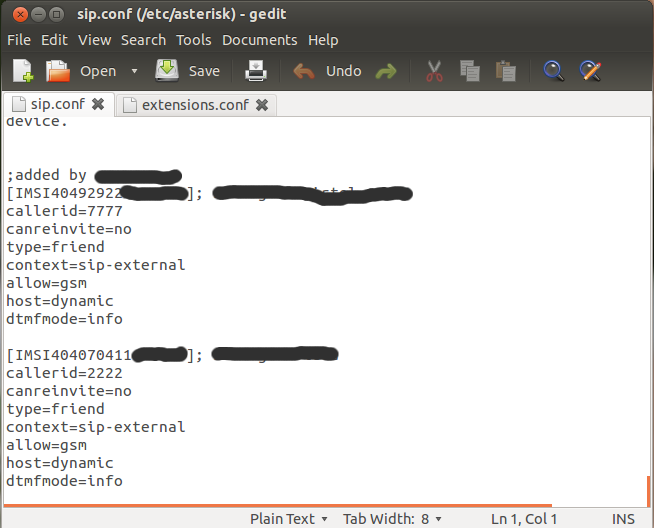
\includegraphics[width=\textwidth]{../images/sip_conf}
  \caption[sip.conf]{Screenshot of \emph{sip.conf}.}
  \label{sip_conf}
\end{figure}

Sip.conf is for user devices configuration. SIP is a session initiation
protocol which is a protocol for call session handling. Sip.conf is a file in
\emph{/etc/asterisk} used to configure SIP devices for communication with the
asterisk system. We have sections for each SIP users also referred to as sip
extensions, in this file. The first option of these sections is the name of
the user device. We have named each user device using the IMSI of the SIM used
by the device. The second option defines the caller ID that we have assigned
to the user. The next option describes the type which we have set as ‘friend’.
This tells that the match will happen first with the name and then the
IP~address. If it is set to ‘peer’ the IP address will be directly matched.
If it is set ‘user’ only the name will be matched directly. Next option is the
context which defines which dial plan from the extension.conf file will be
used. The next option is ‘allow’ which refers to the audio codec that will be
allowed for the call. 

\section{Extension.conf}

\begin{figure}
  \centering
    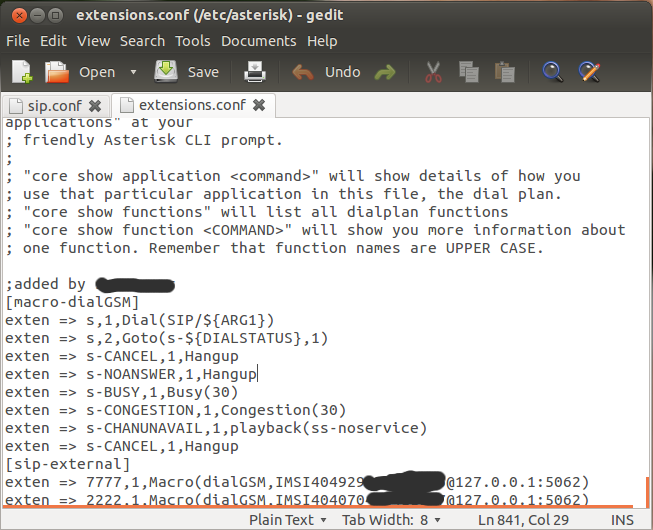
\includegraphics[width=\textwidth]{../images/ext_conf}
  \caption[extensions.conf]{Screenshot of \emph{extensions.conf}.}
  \label{ext_conf}
\end{figure}

This file is  also in there inside etc/asterisk and it consists of the
description of the dial plan. The dial plan defines how the calls flow into
and out of the system, a form of scripting language , the dialplan contains
instructions that asterisk follows in response to external triggers. 
Add following lines at end of the file extension.conf file. We should use
macros to avoid repeating the same dial plan for every client as below.


\begin{verbatim}
[macro-dialGSM]
exten => s,1,Dial(SIP/${ARG1})
exten => s,2,Goto(s-${DIALSTATUS},1)
exten => s-CANCEL,1,Hangup
exten => s-NOANSWER,1,Hangup
exten => s-BUSY,1,Busy(30)
exten => s-CONGESTION,1,Congestion(30)
exten => s-CHANUNAVAIL,1,playback(s-noservice)
exten => s-CANCEL,1,Hangup
\end{verbatim}

Now we define a new context which maps between Caller Id and the IMSI as shown
below. This is needed because when you make a call, you don't dial a
destination IMSI but you call its caller ID.

\begin{verbatim}
[sip-external]
exten => 200,1,Macro(dialGSM,IMSI40420137807462@127.0.0.1:5062)
exten => 202,1,Macro(dialGSM,IMSI404201675035769@127.0.0.1:5062)
\end{verbatim}


\section{sqlite3.db}

\begin{figure}
  \centering
    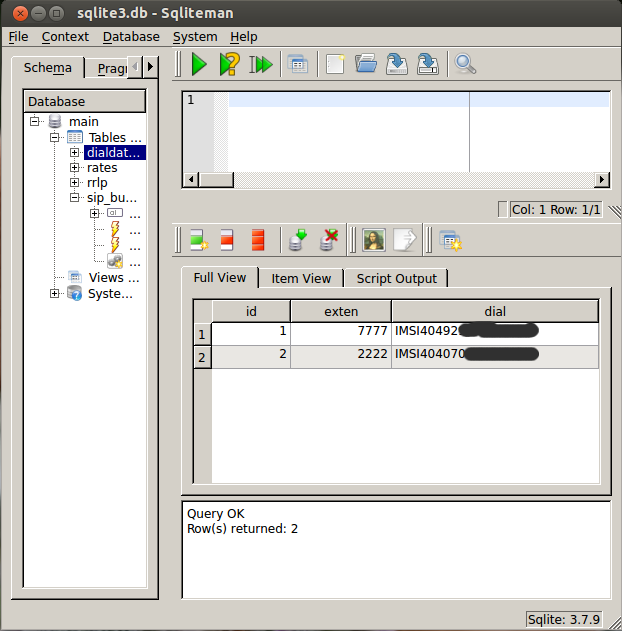
\includegraphics[width=\textwidth]{../images/dialdata}
  \caption[Screenshot - sqlite3.db]{Screenshot of \emph{sqlite3.db}.}
  \label{dialdata}
\end{figure}

Figure \ref{dialdata} is the screenshot of the sqlite3.db file. Sqlite3.db is 
the database in sqlite format. It is part of the asterisk only. There are two
tables in this database. One is dialdatatable and sip\_buddies. 
Dialdatatable contains mapping from IMSI  to the dialing number defined by us.
Sip\_buddies contain user device configuration similar to what we have it 
sip.conf. If we fill up only the dialdatatable and not sip\_buddies during SMS
the IMSI numbers will be shown instead of the SIP usernames (phone numbers)
which is not very convenient.

After doing these specified changes we can call using the registered SIMs
using the local network and also send SMS. More than one pair of users can be
registered in the network. But if two calls happen simultaneously time
division multiplexing is done as OpenBTS can operate only on one frequency
at a time. 
